\documentclass[]{aiaa-tc}% insert '[draft]' option to show overfull boxes

 \usepackage{varioref}%  smart page, figure, table, and equation referencing
 \usepackage{wrapfig}%   wrap figures/tables in text (i.e., Di Vinci style)
 \usepackage{threeparttable}% tables with footnotes
 \usepackage{dcolumn}%   decimal-aligned tabular math columns
  \newcolumntype{d}{D{.}{.}{-1}}
 \usepackage{nomencl}%   nomenclature generation via makeindex
  \makeglossary
 \usepackage{subfigure}% subcaptions for subfigures
 \usepackage{subfigmat}% matrices of similar subfigures, aka small mulitples
 \usepackage{fancyvrb}%  extended verbatim environments
  \fvset{fontsize=\footnotesize,xleftmargin=2em}
 \usepackage{lettrine}%  dropped capital letter at beginning of paragraph
% \usepackage[dvips]{dropping}% alternative dropped capital package
% \usepackage[colorlinks]{hyperref}%  hyperlinks [must be loaded after dropping]
%\usepackage{makeidx}
\graphicspath{{Images/}}

%\usepackage[colorlinks]{hyperref}
%\hypersetup{colorlinks = false}
\usepackage{pdfpages}
\usepackage[ampersand]{easylist}

%AJL SEIT Comment out these two lines for the final submission
%\usepackage{draftwatermark}
%\SetWatermarkFontSize{5cm} \SetWatermarkScale{6} \SetWatermarkText{\textbf{DRAFT-REMOVE}}
\pagestyle{plain}

 \title{Towards Self Driving: Sensing and Learning\\ Interim report}

 \author{
  Michael McDonnell\thanks{CAPT, School of Engineering and Information Technology, ZEIT4901}\
  \\
  {\normalsize\itshape
   UNSW Canberra at ADFA.}\\
  }

 % Data used by 'handcarry' option
 \AIAApapernumber{YEAR-NUMBER}
 \AIAAconference{Conference Name, Date, and Location}
 \AIAAcopyright{\AIAAcopyrightD{YEAR}}

 % Define commands to assure consistent treatment throughout document
 \newcommand{\eqnref}[1]{(\ref{#1})}
 \newcommand{\class}[1]{\texttt{#1}}
 \newcommand{\package}[1]{\texttt{#1}}
 \newcommand{\file}[1]{\texttt{#1}}
 \newcommand{\BibTeX}{\textsc{Bib}\TeX}

%\makeindex

\begin{document}

\maketitle


%\begin{abstract}
%These instructions give you guidelines for preparing your Final Project Summary Report. Use this document as a template if you are using  \LaTeX\ . Otherwise, use this document as an instruction set. The title of this report should be your project title and should NOT contain the word thesis. This section is the abstract, which should concisely summarise your report including the aim, motivations, methodology and observations (or achievements) and conclusions in a single paragraph. Define all symbols used in the abstract. Do not cite references in the abstract. The abstract should be no more than 400 words in length. The footnote on the first page should list your project course. See  \underbar{http://seit.unsw.adfa.edu.au/ojs/index.php/juer} for past examples of final thesis reports, bearing in mind the length requirements may vary.
%\end{abstract}


\tableofcontents
%Anyone know an automated way to do this? Simple as that??!!!!!
%\listoffigures
%\listoftables


%\section*{Nomenclature (examples � include units where appropriate)}
%
%%AJL - COMMENT OUT WHEN YOU WANT TO USE THE AUTOMATIC FILLING OF THE AREA - SEE LATER
%%\printglossary% creates nomenclature section produced by MakeIndex
%\begin{tabbing}
%  XXX \= \kill% this line sets tab stop
%  $J$ \> Jacobian Matrix \\
%  $f$ \> Residual value vector \\
%  $x$ \> Variable value vector \\
%  $F$ \> Force, [N] \\
%  $m$ \> Mass, [kg] \\
%  $\Delta x$ \> Variable displacement vector \\
%  $\alpha$ \> Acceleration, [m/s\textsuperscript{2}] \\[5pt]
%  \textit{Subscript}\\
%  $i$ \> Variable number \\
% \end{tabbing}

\newpage
\section{Introduction (or some other more appropriate heading)} \label{sect:intro}
%\index{}


\lettrine[nindent=0pt]{\textbf{G}}{\textbf{eneral background.}} Autonomous vehicles in general - self driving autopilot etc for personal travel. Relies on mass sensors and data. Wider applications include cognitive assistance and autonomous logistics (refs? Has this been done?). 

\textbf{Other lit review related stuff}

\textbf{Scope and Similar work}. Requirement for robust navigation data. Ability to extend tech requires more agile approach. SIMILAR WORK - MIT local navigation goal \cite{mitLocalNavDriving}. Using CV to align position with map service will allow greater cognitive assistance and automation of tasks without the requirement for significant prior mapping. Benefit -> Augmented reality google maps (eventually autopilot). Automated logistics movements (eg military).

\textbf{Road detection lit review} 
Deep CNN for road detection \cite{deepRoadSegmentation}

\textbf{Autonomous navigation lit review}

\subsection{Project aim}

The aim of this project is to investigate localising navigation data from a GPS feed to the observed road via a vehicle mounted camera. A subordinate aim as part of this is to develop a simulation that will provide sensor data to an external program for processing. 

GPS route data is held as encoded polylines which represents a road as a series of connected points \cite{googleMapPolyline}. The approach for the positional localisation is to use the vehicle GPS position as a fuzzy input location and detected road features to identify an accurate position of the vehicle and identify the GPS route on forward facing video feed. This sets the conditions for autonomous control of the vehicle based on a programmed nagivation route. 

A subordinate aim to the project is the development of a simulation which provides a sensor data, such as location and video feeds from a simulated vehicle. This simulation will allow both the generation of a large and varied data set for testing as well as allow the ability to provide control feedback for the simulated vehicle based off the processing of the sensor data.
\textbf{TODO: Come up with better term than 'external program'. TERMS: External Program, Simulation `tick', Computer vision CV}

The data flow is anticipated to be as follows:
\begin{easylist}[itemize]
	& Simulated sensor data passed to external program
	& External program processes data:
	&& Road/Lane detection
	&& Curve/Map matching of current GPS area
	&& Reprojection of desired direction onto road image
	& External program returns control data (as applicable) to simulation for next `tick'
\end{easylist}

\subsection{Scope and Deliverables}

The scope of the project is deliberately kept constrained initially. This is to focus on the specific problem of localising a navigation route without losing development effort to supporting elements. While the scope is initially narrowly defined it can be extended towards the end of the project as time and opportunity allow.

The scope and deliverables have been identified as follows:
\begin{easylist}[itemize]
	& \textbf{Limitation of road complexity.} There is a requirement for road/lane detection as part of this project (to marry up with the GPS polyline data) however it is not the main focus of the project. Further as the project purely uses the output data of lane detection, it can be considered a `black box' and implementations can be swapped out as more advanced options are identified. The initial limitations on scope of road detection includes:
	&& Limit road detection to easily detectable road surface
	&& Limit roads to single lane
	& \textbf{TODO: OTHER SCOPE?!??!}
	& \textbf{Simulation deliverable requirements.} A core supporting element of this project is the development of the simulation. In addition to providing data for this project the intent is for the simulation to be held as an asset within SEIT for use in subsequent student projects in this area. The basic requirements for the simulation are:
	&& Ability to provide 3D video feed of simulated driving to external program
	&& Support simulated GPS tracking data
	&& Support simulation of GPS route guidance
\end{easylist}



\section{Project management}

\subsection{Project flow}
\textbf{TODO: Cut the extra crap from here - just talk about how it flows in general and leave the rest for the current work part}

The initial state of the project consisted of autonomous vehicles as the general area of focus, as a result the first phase of the project was the identification of the `problem area' and narrowing of scope. A broad reading of relevant research and industry articles identified the ability to navigate in arbitrary areas as a candidate problem area and the scope was refined as outlined in section \ref{sect:intro}. 

This project is being undertaken in an area of study that is a new field for the author. As a result the early focus was on developing base competencies in digital image processing and general computer vision. This included a variety of tools and \textbf{TODO: Talk about the analysis of CV options. This included lane detection}

In parallel with the CV competency development, research and experimentation on key technical risk elements of the simulation was conducted. \textbf{TODO: These include.....}

TODO:  Intersection detection, Curve matching (splines etc) and/or Map matching, 

\subsection{Gantt Chart discussion}

\section{Current work}

\subsection{Computer Vision? Lane Detection}
Before any effective computer vision approaches can be implemented a robust base of understanding of digital image processing is required (What IS CV, DIP). Background study (textbooks, online course etc)

Intent of CV, what are the outcomes (lane detection, intersection detection)

flow - inverse perspective mapping. 
The output of the inverse perspective mapping calibration undertaken is included as figure \ref{f:inverse_perspective_calibration}.

\begin{figure}[htb]% order of placement preference: here, top, bottom
	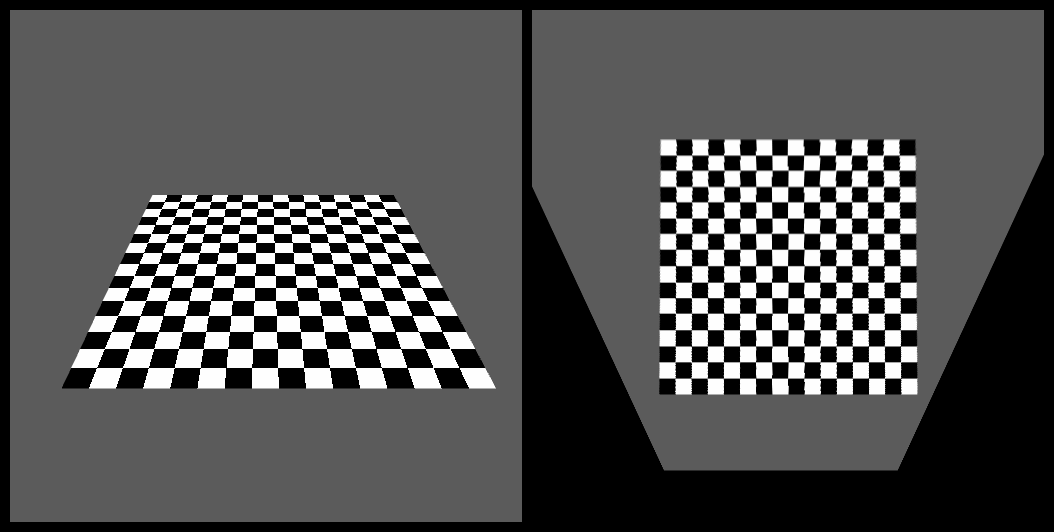
\includegraphics{InversePerspectiveEg.png}
	\caption{Inverse perspective mapping calibration}
	\label{f:inverse_perspective_calibration}
\end{figure}


\subsubsection{Python vs C++}

\subsubsection{Open CV}
Digital Image Processing course, Open CV vs from scratch

\subsubsection{Alternate approaches to lane detection}
CNN discussion with references?

\subsection{Simulation system}
Intent of simulation
IPC

\subsubsection{Simulation engine}
%Home rolled vs Unreal (C++ so can talk direct to OpenCV C++) vs Unity 


\subsubsection{Interprocess Communication (IPC)}

One of the main issues identified with using Python Open CV and the Unity game engine is the ability for simulation data, for example video feeds, to be transferred from Unity to the Python process. This was a significant technical challenge (REF GANTT CHART? HOW LONG WAS BUDGETED). The motivation for fast IPC was to allow real time processing of the simulation data in order to allow for potential control feedback to the simulation. Transferring image data represents a large amount of memory thus has a significant time complexity per simulation `tick'. 

The initial research approach involved investigating the ability to use a static memory buffer that could be written to by Unity and read by Python. Shared memory or memory mapped files do offer this however they add another level of complexity and implementation details are largely for lower level languages and could not be identified in particular for Python. Named pipes were also investigated and, while they represented an improved option, still had many of the technical and implementation complexity issues of the memory mapped approach.

The final solution identified was using TCP via the ZeroMQ middleware. This has implementations for both C\# and Python and is well optimised for speed on localhost (\textbf{TODO: What is localhost}) machines. The speed of this approach is highly dependant on the size of the transferred data \textbf{TODO: GRAPH OF TIME PERFORMANCE OF 64, 128, 256 AND 512....}. The use of this approach requires slower than real time simulation processing which was achieved by dynamic simulation time dilation, discussed in section \ref{sect:timedilation}. This approach allows easy and reliable two way communication which is required for effective feedback between the processes. This is something that would be complicated significantly by memory mapping, requiring multiple memory locations with varying roles. The current solution also offers the ability to expand off a single local machine, for example a hosted simulation with remote processing. While this is well out of scope of this thesis it presents additional flexibility for future development.

Once the IPC approach was confirmed, the data handling pipeline between the Unity (C\#) and Python processes was developed. The final simulation output data structure for video feed is a flattened 3D byte array, consisting of the x and y pixel coordinates and the colour value. The colour is represented by a four element vector of bytes for the Red, Blue, Green and Alpha channels. 

The Python process casts the byte stream as a byte array and reshapes the data to a 3D array. The fourth element of each colour value is removed, resulting in a final data structure consisting of a 2D array of 3 element vectors of bytes which is the required data structure for OpenCV processing operations. 

A simple calibration was established using three coloured cubes (Red, Green and Blue) in Unity to confirm colour channel and axis orientation correctness. A still from the colour image IPC calibration undertaken is included as figure \ref{f:unity_calibration}. \textbf{TODO: Fix image - border? Also shrink and put in/near text}

\begin{figure}[htb]% order of placement preference: here, top, bottom
 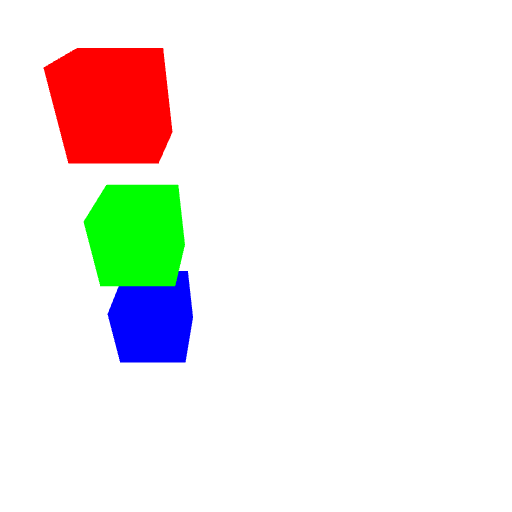
\includegraphics{unity_calibration.png}
 \caption{Still from calibration of colour image IPC pipeline between Unity and Python}
 \label{f:unity_calibration}
\end{figure}


\subsubsection{Simulation time dilation}\label{sect:timedilation}

It was determined that the simulation had a requirement to dynamically scale simulation time based on the external processing in order to ensure the simulation effectiveness regardless of the data processing time requirement. \textbf{TODO: Allows }

\section{Results}
Is this required?
\subsection{Computer vision}


\section{Future work}

\subsection{Lane line detection}

Detect the curve of the lane and identify intersections
Curve detection options - sliding window REF LINK %https://www.spiedigitallibrary.org/conference-proceedings-of-spie/0852/0000/Progress-In-Road-Intersection-Detection-For-Autonomous-Vehicle-Navigation/10.1117/12.968232.short?SSO=1


%
%\begin{table}[t] % no placement specified: defaults to here, top, bottom, page
% \begin{center}
%  \caption{Expectations for the Assessment of the Final Project Summary Report \
% (Final Project Summary Report is worth 35\% of the course) }
%  \label{t:scheme_marking}
%  \begin{tabular}{|c|} \hline
%\\
%\textbf{Understanding of the topic: (What and why?)} \\\hline
%�	Has the problem been adequately defined? \\
%�	Has a critical review of the relevant literature been performed? \\
%Note the most important references should be included in this report, whereas \\
%extensive literature reviews where appropriate should be confined to the \\
%Appendices or your separate Project Specific Deliverable. \\
%�	Has the relationship between the project and the literature been adequately defined? \\
%�	Has a clear, appropriate and attainable set of aims been identified? \\
%\\
%\textbf{Methodology (How?)}  \\\hline	
%�	Has a logical process been developed to meet the aims? \\
%�	Has this process been justified? \\
%�	Is the methodology appropriate for the scope of the project? \\
%\\
%\textbf{Analysis}	 \\\hline
%�	Has there been an adequate collection of data/information (or efficient design)? \\
%�	Has appropriate and sufficient analysis been performed to reduce it to a useful form? \\
%�	Have the aims been adequately addressed (if not then have valid reasons been given)? \\
%\\
%\textbf{Discussion, conclusions and recommendations:} \\\hline	
%�	Are they meaningful/worthwhile/significant within the scope of the project? \\
%�	Are they appropriate and adequately justified? \\
%\\
%\textbf{Presentation of the project report:}	 \\\hline
%�	Is the document set out clearly and logically? \\
%�	Does the text clearly explain all aspects of the project to even a non-expert? \\
%�	Has appropriate use been made of figures/tables/charts? \\
%�	Has appropriate and accurate use of referencing been made? \\
%\\
%\textbf{Management}	 \\\hline
%�	There is no requirement for an explicit management document, but it may be \\
%appropriate for you to briefly discuss your learnings in terms of expectations \\
%in the context of your project. \\
%\\
% \\\hline
% \end{tabular}
% \end{center}
%\end{table}



%\begin{figure}[htb]% order of placement preference: here, top, bottom
% 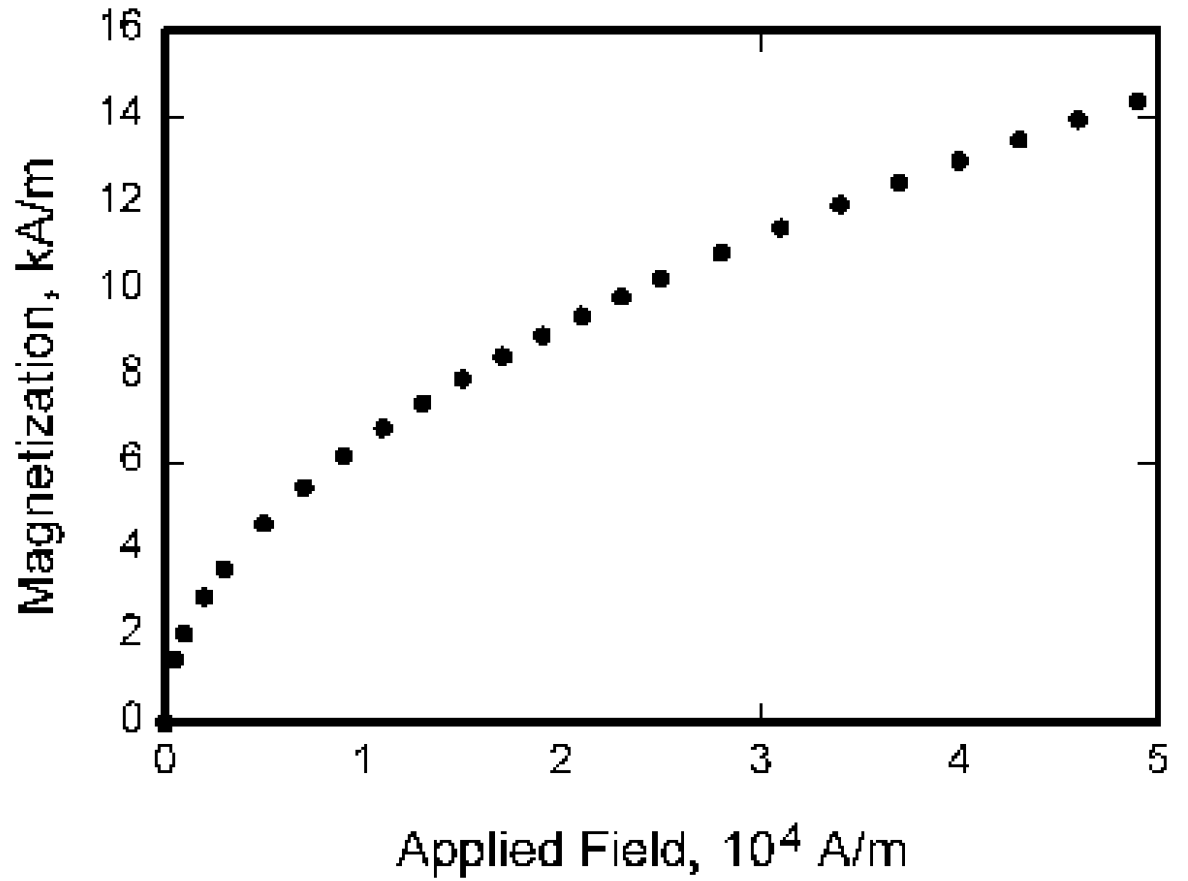
\includegraphics{image_eg.png}
% \caption{Magnetization as a function of applied field, which has
%   borders so thick that they overwhelm the data and for some reason the
%   ordinate label is rotated 90 degrees to make it difficult to
%   read. This figure also demonstrates the dangers of using a bitmap
%   as opposed to a vector image.}
% \label{f:magnetic_field}
%\end{figure}

%Sometimes writing meaningless text can be quiet easy, but other times one is hard pressed to keep the words flowing.\footnote{And sometimes things get carried away in endless detail.}
%
%\begin{table}% no placement specified: defaults to here, top, bottom, page
% \begin{center}
%  \caption{Variable and Fixed Coefficient Runge-Kutta Schemes as a
%           Function of Reynolds Number}
%  \label{t:scheme_comparison}
%  \begin{tabular}{rrr}
%       Re & Vary & Fixed \\\hline
%        1 &  868 & 4,271 \\
%       10 &  422 & 2,736 \\
%       25 &  252 & 1,374 \\
%       50 &  151 &   736 \\
%      100 &  110 &   387 \\
%      500 &   85 &   136 \\
%    1,000 &   77 &   117 \\
%    5,000 &   81 &    98 \\
%   10,000 &   82 &    99
%  \end{tabular}
% \end{center}
%\end{table}

%\subsubsection{Equations, Numbers, Symbols, and Abbreviations}
%Equations are centered and numbered consecutively, with equation numbers in parentheses flush right, as in  Eq.~(\ref{e:function}) that demonstrates some math
%typesetting.

%\begin{equation}
% \label{e:function}
% \int_{0}^{r_{2}} F(r,\varphi) \, dr \, d\varphi =
%    \left[ \sigma r_{2}/(2\mu_{0}) \right] \cdot
%    \int_{0}^{\infty} \exp(-\rho|z_{j}-z_{i}|) \, \lambda^{-1} 
%\end{equation}
%Eq.~(\ref{e:function}) is grand.
%
%
\section{Conclusions}
The conclusions should summarise the main findings of your thesis project including a brief reference to the supporting evidence and to the initial aims. Note that the Conclusions and Recommendations sections are the last sections of the paper that should be numbered. The acknowledgements and references should be listed without numbers.
This had been a brief example of some of the more advanced options available for \LaTeX\ .

\section{Recommendations}
This section should discuss and recommend directions for future work that will build on and extend your research and perhaps resolve some of the issues that you have encountered in your work.

\section*{Acknowledgements}
The Acknowledgements section should be used to briefly thank those individuals or organisations that have assisted you directly in your thesis work whether they be family, friends and colleagues, or technical and academic staff. Note that any external funding source that supported your project should be acknowledged here. 

\section*{Appendices (Separate Document)}
Appendices may used to archive detailed summaries of data such as images, tables and charts and detailed example calculations such as for the estimation of measurement uncertainty. They may also include design drawings. Raw data, or detailed computer programs and files and extensive design drawings, should not be included. Their archiving should be discussed with your supervisor. Any appendices should be submitted as a SINGLE separate document file if referred to in the main text and be listed in the table of contents at the beginning (Note the use of a separate page numbering scheme).

% If you use MakeIndex
%\printindex


% AJL - UNCOMMENT THIS IS PREFERENCE TO THE ABOVE SECTION
%% produces the bibliography section when processed by BibTeX
\bibliography{InterimReferences}
\bibliographystyle{aiaa}

\appendix
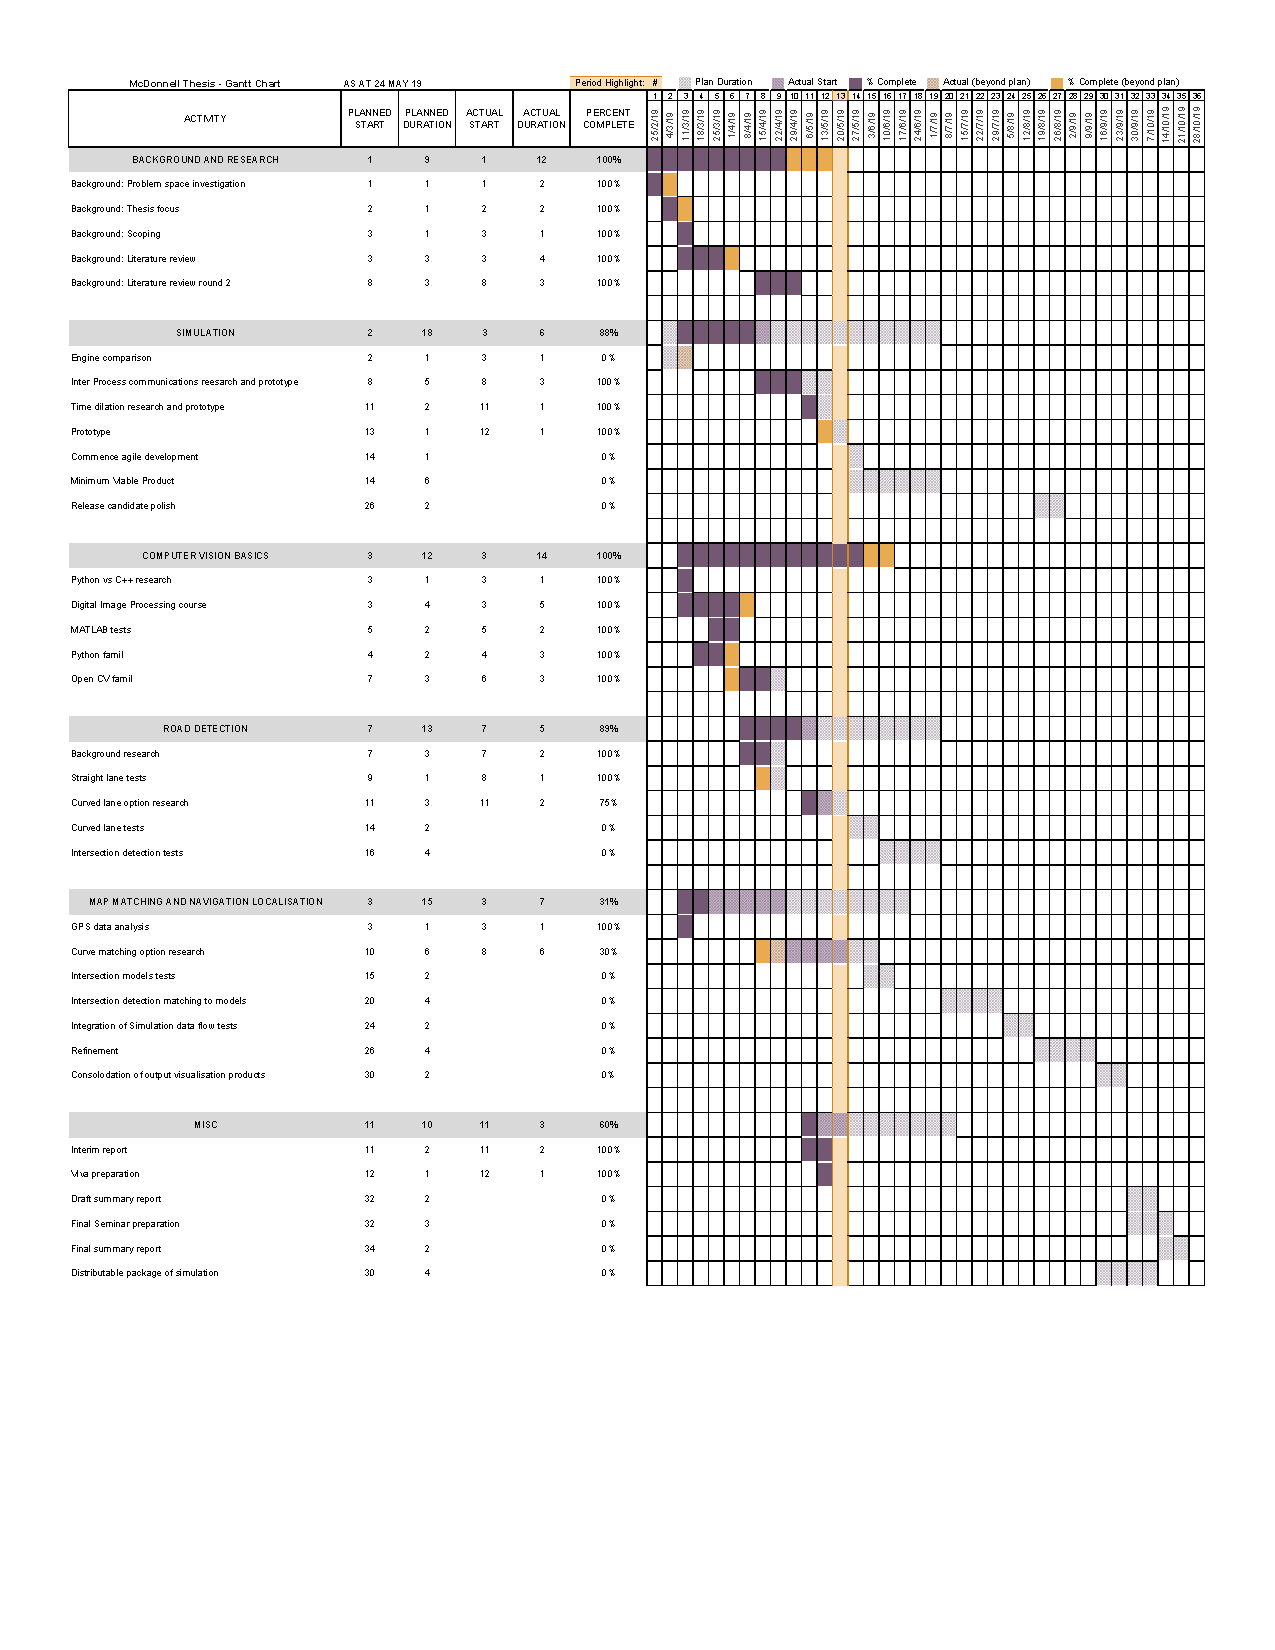
\includepdf[angle=-90,scale=0.9,pages=1,pagecommand=\section{Gantt Chart for Research Project}]{GanttChart.pdf}


\end{document}

